\usetikzlibrary{arrows.meta,decorations.pathreplacing,patterns}

\begin{frame}{fair (de)queuing}
    \begin{tikzpicture}
        \foreach \x in {0,1,2,5,7,8} {
            \path[fill=violet!30] (\x, -.5) rectangle ++(1, 1);
        }
        \foreach \x in {3,4,6} {
            \path[pattern=checkerboard,pattern color=blue!70!black]
                (\x, -.5) rectangle ++(1, 1);
        }
        \foreach \x in {1,2,3,4,5,6,7,8} {
            \draw (\x, -.5) -- (\x, .5);
        }
        \draw (0, -.5) rectangle (9, .5);
        \draw[ultra thick,-Latex] (9, 0) -- 
            (10, 0) to[out=0,in=90] (11, -.5)
            to[out=-90,in=0] (10, -1) -- (0, -1)
            to[out=180,in=90] (-1, -1.5)
            to[out=-90,in=180] (0, -2);

        \draw[very thick] (-.25, -1.5) -- (13, -1.5);
        \draw[very thick] (-.25, -2.5) -- (13, -2.5);
            \begin{scope}
            \clip (-.25, -1) rectangle (13, -3);
            \foreach \x in {0,2,4,6,7,8} {
                \path[draw,fill=violet!30] (-0.0 + \x * 1.5, -2.4) rectangle ++(1.5, 0.8);
            }
            \foreach \x in {1,3,5} {
                \path[draw,pattern=checkerboard,pattern color=blue!70!black] (-0.0 + \x * 1.5, -2.4) rectangle ++(1.5,0.8);
            }
            \end{scope}
        \begin{visibleenv}<2>
            \draw[red,line width=.8mm,decorate,decoration={brace,mirror,amplitude=2mm}]
                (0 +0.1, -2.6) -- (6 * 1.5 -0.1, -2.6)
                    node[midway,below=3mm,align=center] {alternate (`round robin') \\ when possible };
            \draw[red,line width=.8mm,decorate,decoration={brace,mirror,amplitude=2mm}]
                (6 * 1.5 +0.1, -2.6) -- (13 -0.1, -2.6)
                    node[midway,below=3mm] {always keep link busy};
        \end{visibleenv}
    \end{tikzpicture}
\end{frame}

\begin{frame}{problem 1: variable packet size}
    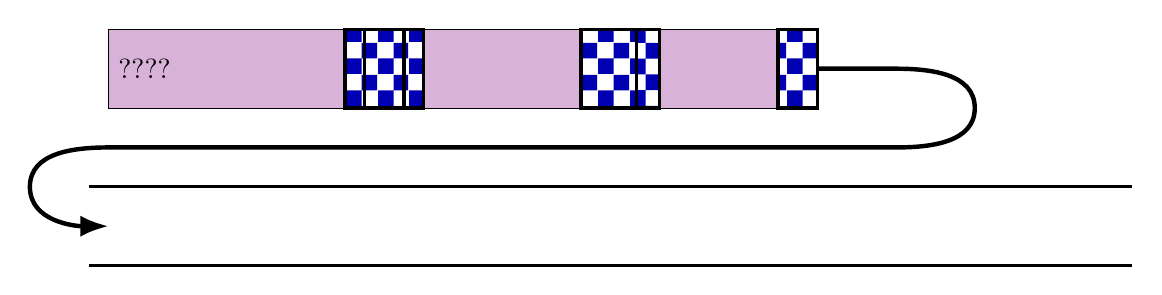
\begin{tikzpicture}
        \foreach \x/\sz in {0/3,4/2,7/1.5} {
            \path[draw,fill=violet!30] (\x, -.5) rectangle ++(\sz, 1);
        }
        \foreach \x/\sz in {3/.25,3.25/.5,3.75/.25,6/.7,6.7/.3,8.5/0.5} {
            \path[draw,very thick,pattern=checkerboard,pattern color=blue!70!black]
                (\x, -.5) rectangle ++(\sz, 1);
        }
        \draw (0, -.5) rectangle (9, .5);
        \draw[ultra thick,-Latex] (9, 0) -- 
            (10, 0) to[out=0,in=90] (11, -.5)
            to[out=-90,in=0] (10, -1) -- (0, -1)
            to[out=180,in=90] (-1, -1.5)
            to[out=-90,in=180] (0, -2);

        \draw[very thick] (-.25, -1.5) -- (13, -1.5);
        \draw[very thick] (-.25, -2.5) -- (13, -2.5);
        \node[anchor=west] (1, -3) {????};
    \end{tikzpicture}
    \begin{itemize}
        \item just alternating packets doesn't work with variable sizes
        \item need to send more packets from flows with faster packets
    \end{itemize}
\end{frame}

% FIXME
\begin{frame}{problem 2: packets arriving late}
\small
\begin{tabular}{lll}
time = & queue & \\
 & A1, B1, B2, B3 & \\
0.0 & B1, B2, B3 & start sending A1 \\
1.0 & B1, B2, B3 & finish sending A1 \\
1.0 & B2, B3 & start sending B1 \\
2.0 & B2, B3 & finish sending B1 \\
2.0 & B3 & start sending B2 \\
2.1 & B3, A2 & receive A2 \\
2.9 & B3, A2, A3 & receive A3 \\
3.0 & B3, A2, A3 & finish sending B2 \\
\end{tabular}
\begin{itemize}
\item<2-> flow A missed a turn because packet was just a little late
\item<2-> intuition: should get extra turn to make up for this?
\end{itemize}
\end{frame}

